
The testing described in Section \ref{sec:randerr} describes the process of
evaluating the methodology with test cases drawn from the training database.
It is also helpful to test the methodology against real assays of \gls{SNF}.
The \gls{SFCOMPO} database was created to allow access to these sorts of
measurements linked to the reactor operation parameters being predicted in this
work \cite{sfcompo, valid_sfco}. The only parameter not part of the
\gls{SFCOMPO} database is the time since irradiation, so that is not predicted
here. 

\begin{figure}[!htb]
  \centering
  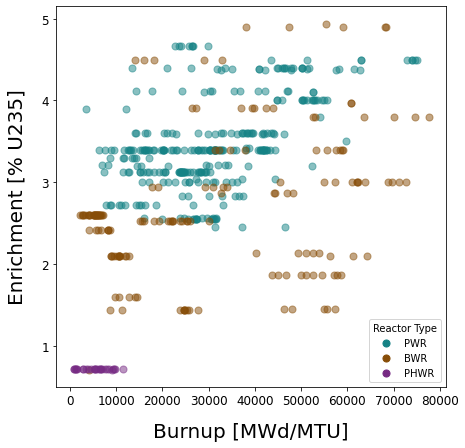
\includegraphics[width=0.7\textwidth]{./chapters/exp1/sfcompo_scatter_viz.png}
  \caption[Scatter plot of distribution of \acrshort{SFCOMPO} testing set 
           labels]
          {Scatter plot showing the range of reactor operation parameters in 
           the \acrshort{SFCOMPO} testing set that are being predicted.}
  \label{fig:sfcoscatter}
\end{figure}

The database used in this work is a filtered version of all the entries in the
original database. First, only the nuclide concentration measurements are kept
so that the training set measurements could be converted to the units in
\gls{SFCOMPO}.  The assays in \gls{SFCOMPO} are presented as nuclide
concentrations with the units milligrams per grams of initial uranium, or
$mg/gU_i$. The training set of nuclide measurements in $grams$ is converted to
these concentration units prior to prediction is converted to these
concentration units prior to prediction. Second, only the \gls{PWR}, \gls{BWR},
and \gls{PHWR} entries are retained and all other reactor types are excluded.
Third, uranium-gadolinium fuels are not simulated in the training set and
therefore are also removed from the testing set. Last, duplicate entries for
some measurements exist and the first entry is kept in these cases. 

In all, there are 505 test cases that are able to compare against the training
database.  The number of each reactor type is as follows: 312 \glspl{PWR}, 165
\glspl{BWR}, and 28 \glspl{PHWR}. The space of enrichment and burnup values
is visualized in Figure \ref{fig:sfcoscatter}. These are sufficiently
represented in the training set design, as pictured in Figure
\ref{fig:trainhist}, although the proportions of \gls{PWR} and \gls{BWR} are
approximately opposite to the training set. 

There is one main issue with using \gls{SFCOMPO} as a testing set: missing
nuclide measurements.  The feature set of 29 nuclides in Table
\ref{tbl:nucmass} was chosen based on the frequency of these measurements being
present in the database at an arbitrary level of 100 measurements. This
happened before filtering the uranium-gadolinium fuel, so there are some
nuclide measurements present at under 100 counts.  Each nuclide's frequency in
\gls{SFCOMPO} is listed in Table \ref{tbl:missing}.  While every assay contains
several plutonium measurements and most contain uranium measurements as well,
the remaining nuclides are present at a much lower rate. 

\begin{table}[!htb]
  \centering
  \begin{tabular}{>{\raggedleft}m{0.6in}
                                m{0.4in}
                  >{\raggedleft}m{0.6in}
                                m{0.4in}
                  >{\raggedleft}m{0.6in}
                                m{0.4in}}
    \toprule
    \rowcolor[gray]{0.88} ${}^{241}\text{Am}$  & 237 & ${}^{145}\text{Nd}$ & 162 & ${}^{147}\text{Sm}$ & 97  \\  
    \rowcolor[gray]{0.95} ${}^{242m}\text{Am}$ & 110 & ${}^{146}\text{Nd}$ & 139 & ${}^{149}\text{Sm}$ & 97  \\ 
    \rowcolor[gray]{0.88} ${}^{243}\text{Am}$  & 203 & ${}^{148}\text{Nd}$ & 275 & ${}^{150}\text{Sm}$ & 97  \\ 
    \rowcolor[gray]{0.95} ${}^{242}\text{Cm}$  & 214 & ${}^{150}\text{Nd}$ & 121 & ${}^{151}\text{Sm}$ & 97  \\ 
    \rowcolor[gray]{0.88} ${}^{244}\text{Cm}$  & 269 & ${}^{237}\text{Np}$ & 155 & ${}^{152}\text{Sm}$ & 97  \\ 
    \rowcolor[gray]{0.95} ${}^{134}\text{Cs}$  & 113 & ${}^{238}\text{Pu}$ & 369 & ${}^{234}\text{U}$  & 355 \\ 
    \rowcolor[gray]{0.88} ${}^{137}\text{Cs}$  & 185 & ${}^{239}\text{Pu}$ & 505 & ${}^{235}\text{U}$  & 479 \\ 
    \rowcolor[gray]{0.95} ${}^{154}\text{Eu}$  & 100 & ${}^{240}\text{Pu}$ & 505 & ${}^{236}\text{U}$  & 462 \\ 
    \rowcolor[gray]{0.88} ${}^{143}\text{Nd}$  & 162 & ${}^{241}\text{Pu}$ & 504 & ${}^{238}\text{U}$  & 433 \\ 
    \rowcolor[gray]{0.95} ${}^{144}\text{Nd}$  & 113 & ${}^{242}\text{Pu}$ & 505 &       &     \\ \bottomrule
  \end{tabular}
  \caption[Number of assays each nuclide is measured for in \acrshort{SFCOMPO}]
          {Number of assays each nuclide is measured for in the 
           \acrshort{SFCOMPO} database.}
  \label{tbl:missing}
\end{table}

Although some algorithms in theory can handle null values in the testing stage,
scikit-learn does not currently include this capability. The \gls{MLL} method
is designed to handle null values, however. This is done by converting them to
zero and filtering out all zero-valued nuclides during the likelihood
calculations. But there is a technique more commonly applied than imputing
missing values with zero. This involves taking the mean or median of the
existing feature measurements in the testing set and applying that value to the
assays in which it is missing.  The remainder of this section discusses using
the three algorithms to predict the \gls{SFCOMPO} test cases where the nulls
are both imputed using zero and the mean.

\subsubsection{Reactor Type Classification}

Table \ref{tbl:sfcorxtr} presents two metrics for the two missing value
techniques: the accuracy and balanced accuracy scores. The accuracy scores for
both the mean-imputed nulls and zero-imputed nulls test sets are mostly under
0.62, which is the fraction of \gls{PWR} entries.  Therefore, a classifier
could predict \gls{PWR} every time and do better than these accuracy scores.
For the zero-imputed nulls test set predictions using \gls{MLL}, however, the
accuracy of 0.72 does exceed the "majority guess" accuracy of 0.62.  Since
\gls{MLL} calculations filter out null values, it is expected that the scores
will be higher for all prediction categories where \gls{MLL} is being used with
the zero-imputed nulls test set. This expected \gls{MLL} performance also holds
true when looking at the balanced accuracy score.  A balanced accuracy score of
0 denotes random guessing, but it can also be negative if the classifications
are worse than random guessing. The balanced accuracy of 0.63 for the
zero-imputed nulls case is a promising result. The balanced accuracies of
\textit{k}-nearest neighbors and decision trees are all quite low. Also, the
higher accuracies correspond to lower balanced accuracies, and vice versa.
Therefore, further investigation is necessary.

\begin{table}[!htb]
  \centering
  \begin{tabular}{@{}m{1.5in}llllll@{}}
    \toprule
    & \multicolumn{3}{m{2in}}{Accuracy Scores} 
    & \multicolumn{3}{l}{Balanced Accuracy Scores} \\ 
    \toprule
    Null Handling    & kNN   & DTree  & MLL   & kNN   & DTree  & MLL    \\ \midrule
    Mean Imputation  & 0.52  & 0.60   & 0.39  & 0.09  & 0.12   & -0.01  \\
    Zero Imputation  & 0.45  & 0.42   & 0.72  & 0.21  & 0.30   & 0.63   \\ \bottomrule
    \end{tabular}
  \caption[Performance of reactor type classification of \acrshort{SFCOMPO} 
           entries]
          {Accuracy and balanced accuracy scores for reactor type prediction 
           of the \acrshort{SFCOMPO} test cases.}
  \label{tbl:sfcorxtr}
\end{table}

\begin{figure}[!htb]
  \centering
  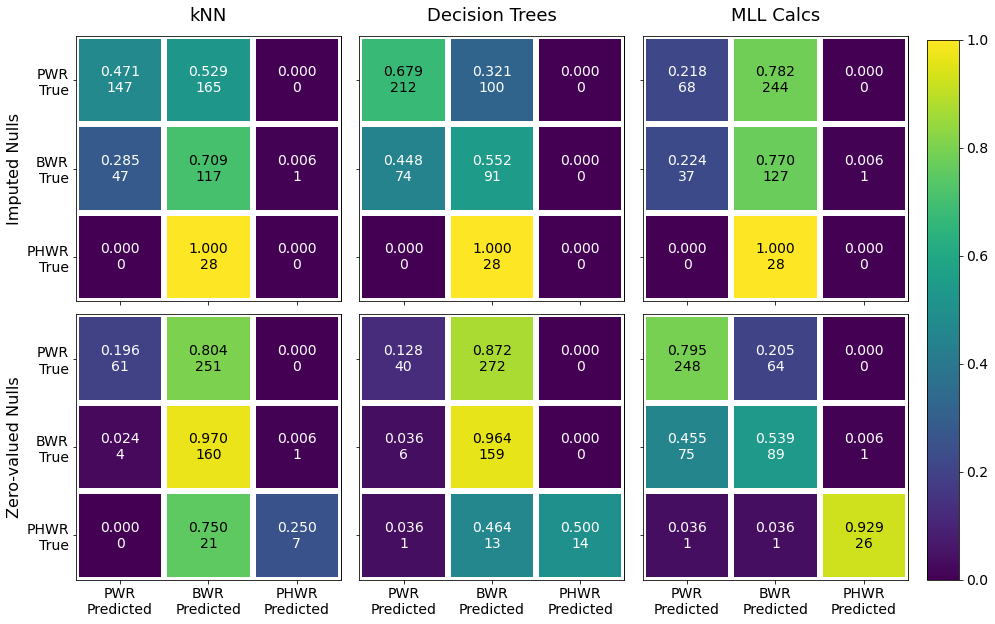
\includegraphics[width=\textwidth]{./chapters/exp1/confusion_matrix_sfco.png}
  \caption[Confusion matrices of reactor type classification of 
           \acrshort{SFCOMPO} entries]
          {Confusion matrices of reactor type prediction for each algorithm 
           using two missing entry techniques: imputation with mean values (top 
           panel) and with zero (bottom panel).}
  \label{fig:cm}
\end{figure}

Figure \ref{fig:cm} allows for a deeper look into what is happening with the
reactor type predictions for both of the \gls{SFCOMPO} test sets by studying
the confusion matrices, which are introduced in Sections \ref{sec:testerr} and
\ref{sec:randerrA}.  The matrices from using mean-imputed null values are in
the top panel and the matrices from using zero-imputed null values are in the
bottom panel.  The scikit-learn algorithms have a higher accuracy for the
mean-imputed test set than their zero-imputed counterparts, but the balanced
accuracies follow the opposite direction. For \textit{k}-nearest neighbors,
mean-imputed nulls cause more than half of the \gls{PWR}s and all of the
\gls{PHWR}s to be misclassified as \gls{BWR}s. Additionally, 28.5\% \gls{BWR}s
are misclassified as \gls{PWR}s.  For the zero-imputed nulls test set, there is
a much larger correct \gls{BWR} classification percentage, but also a much
larger \gls{PWR} misclassification percentage. The \gls{PHWR} true positive
percentage increases from 0 to 25\%.  \Gls{BWR} (32\% of test cases) and
\gls{PHWR} (5.5\% of test cases) are the two minority classes in the database.
Because they both have higher true positive fractions but there were overall
fewer correct predictions (from a much higher \gls{PWR} misclassification) from
the mean-imputed nulls to the zero-imputed nulls, the accuracy decreased but
the balanced accuracy increased.

Decision trees follows a similar pattern the the \textit{k}-nearest neighbors
example.  The \gls{PWR} misclassification increases from the mean-imputed nulls
to the zero-imputed nulls test set in a similar manner, although the original
\gls{PWR} true positive fraction is higher (leading to a higher accuracy for
the mean-imputed nulls case).  As before, the \gls{BWR} correct classification
increases drastically from the mean-imputed nulls to zero-imputed nulls case.
Additionally, the \gls{PHWR} classification improvement from mean-imputed nulls
to zero-imputed nulls is better for decision trees than for \textit{k}-nearest
neighbors.  Therefore, again, the accuracy decreased and the balanced accuracy
increased.  The larger improvement for the minority classes has led to the
larger balanced accuracy improvement for decision trees.

In Figure \ref{fig:cm}, the confusion matrices for the \gls{MLL} calculations
tell a very different story than those for the scikit-learn algorithms.  The
only similarity is that using mean-imputed nulls causes all \gls{PHWR}s to be
classified as \gls{BWR}s. \gls{PWR}s are misclassified as \gls{BWR}s at 78.2\%,
and \gls{BWR}s are misclassified as \gls{PWR}s at 22.4\%. For the zero-imputed
nulls test set, \gls{PHWR}s and \gls{PWR}s true positive percentages sharply
improve to 92.9\% and 79.5\%, respectively.  The true positive rate for
\gls{BWR}s, however, decreases from 77.0\% to 53.9\%. This is the opposite
trend from both of the scikit-learn algorithms.  Despite the misclassification
increase for \gls{BWR}s, both the accuracy score and balanced accuracy score
increase for \gls{MLL} calculations when moving from using mean-imputed null
values to zero-imputed null values in the test set. The improvement in
\gls{MLL} classification is likely because the mean-imputed nulls test set
hides information rather than removing it from consideration, which is what the
zero-imputed nulls test set does. 

All three algorithms using both test sets tend towards misclassifying
\gls{PHWR}s as \gls{BWR}s (except for \gls{MLL} calculations using zero-imputed
null missing values).  This is likely because \gls{BWR}s comprise the majority
of the training set (72\%), and no matter how the missing measurements are
handled there may be too little information to predict these well with most
algorithms.  For the two scikit-learn algorithms, the zero-imputed nulls test
set predicts \gls{BWR}s the majority of the time (despite there being 50\%
correct \gls{PHWR} prediction for decision trees). This also is likely from
\gls{BWR} being the training set majority class, so with many nuclides
measuring at zero, there are likely to be few good matches, and the majority
class becomes the most likely prediction. This explanation is possibly
applicable to the mean-imputed nulls test set as well, but the behavior pattern
is less clear because the mean-imputed nulls give more information for these
algorithms than zero-imputed nulls (since the zero-imputed values cannot be
removed from consideration), so a larger proportion of \gls{PWR}s are being
predicted properly.  

\subsubsection{Regression Cases}
\label{sec:sfcoreg}

Next, the prediction of \gls{SFCOMPO} test samples for the regression cases
will be discussed. There is no time since irradiation value in the database, so
only burnup and \gls{U235} enrichment are discussed here.  While the mean and
median errors for burnup and enrichment prediction are listed in Tables
\ref{tbl:sfcoburn} and \ref{tbl:sfcoenri}, respectively, there are also box
plots included for both absolute and relative errors in Figures
\ref{fig:sfcoburn} and \ref{fig:sfcoenri}, respectively.  Box plots were chosen
since they can provide a larger amount of information than just a mean or
median value.  The white triangles represent the mean error, and the white line
in notched box is the median error. The box itself is the 25\% (Q1) and 75\%
(Q3) quartiles at the bottom and top, respectively. The error bars or whiskers
are meant to represent the spread of all errors minus the outliers.  The bottom
whisker reaches to $Q1 - 1.5(Q3-Q1)$ and the top whisker reaches to $Q3 +
1.5(Q3-Q1)$. Any values outside of the total whisker range, $4(Q3-Q1)$, are
considered outliers. \cite{matplotlib} Lastly, there are plots of the true
value versus the predicted value for both burnup and enrichment in Figures
\ref{fig:yvy_sfcoburn} and \ref{fig:yvy_sfcoenri}, respectively.

\noindent \textbf{Burnup}

The expected results that \gls{MLL} will perform better with the zero-imputed
nulls test set also holds true for the regression cases, as shown in Table
\ref{tbl:sfcoburn}.  While the scikit-learn algorithms have a moderate increase
in both the mean and median burnup errors from the mean-imputed nulls to the
zero-imputed nulls, the \gls{MLL} calculations have an order of magnitude
decrease in error when moving in that same direction.  Seeing this trend
between Figures \ref{fig:burnimp} and \ref{fig:burn0} is a little difficult due
to the different ranges on the vertical axes, but the drastic improvement in
\gls{MLL} burnup error from the mean-imputed nulls in Figure \ref{fig:burnimp}
to the zero-imputed nulls in Figure \ref{fig:burn0} is still visually clear. In
the latter figure, there is one outlier for \textit{k}-nearest neighbors and 39
for \gls{MLL} calculations.

\begin{table}[!htb]
  \centering
  \begin{tabular}{@{}m{1.5in}llllll@{}}
    \toprule
                     & \multicolumn{3}{m{2in}}{Mean Errors $[GWd/MTU]$} 
                     & \multicolumn{3}{c}{Median Errors $[GWd/MTU]$} 
                     \\ \toprule
    Null Handling    & kNN   & DTree & MLL   & kNN   & DTree & MLL    \\ \midrule
    Mean Imputation  & 9.43  & 10.89 & 13.17 & 7.26  & 8.28  & 10.84  \\
    Zero Imputation  & 14.88 & 15.18 & 3.53  & 11.47 & 8.79  & 1.70   \\ \bottomrule
  \end{tabular}
  \caption[Performance of burnup regression of \acrshort{SFCOMPO} entries]
          {Mean and median errors for burnup prediction of the 
          \acrshort{SFCOMPO} test cases.}
  \label{tbl:sfcoburn}
\end{table}

Although the mean and median errors are contained in the range of 
$1-15\:GWd/MTU$, the large spread in burnup errors in Figures \ref{fig:burnimp}
and \ref{fig:burn0} for all three algorithms was broad enough to warrant an
investigation into the range of relative errors, expressed as percent errors in
Figures \ref{fig:burnimppct} and \ref{fig:burn0pct}.  In Figure
\ref{fig:burnimppct} there are 75, 72, and 73 outliers (all around 15\% of the
test database) for the \textit{k}-nearest neighbors, decision trees, and
\gls{MLL} calculations, respectively.  In Figure \ref{fig:burn0pct} there are
45 outliers for the \gls{MLL} calculations.

\begin{figure}[!htb]
  \centering
  \begin{subfigure}[b]{0.49\textwidth}
    \centering
    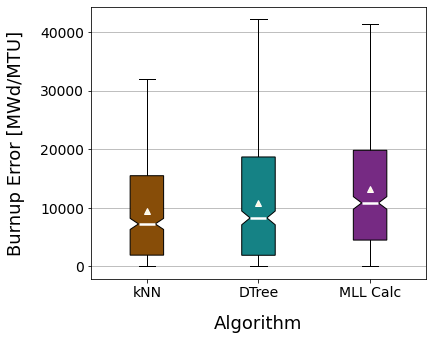
\includegraphics[width=\textwidth]{./chapters/exp1/sfcompo_boxplots_impnull_burn.png}
    \caption{Box plots of burnup errors using mean-imputed null values.}
    \label{fig:burnimp}
  \end{subfigure}
  \hfill
  \begin{subfigure}[b]{0.49\textwidth}
    \centering
    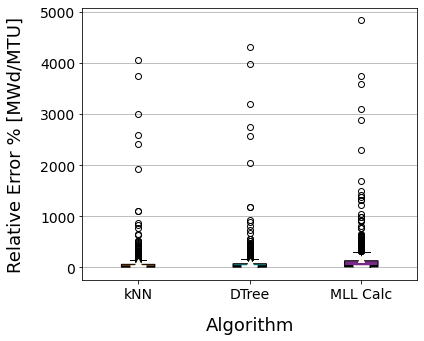
\includegraphics[width=\textwidth]{./chapters/exp1/sfcompo_boxplots_impnull_pcterr_burn.png}
    \caption{Box plots of burnup percentage errors using mean-imputed null values.}
    \label{fig:burnimppct}
  \end{subfigure}
  \vskip\baselineskip
  \begin{subfigure}[b]{0.49\textwidth}
    \centering
    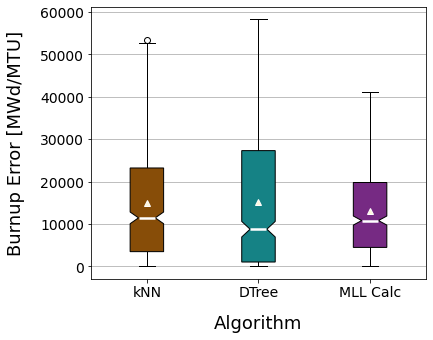
\includegraphics[width=\textwidth]{./chapters/exp1/sfcompo_boxplots_0null_burn.png}
    \caption{Box plots of burnup errors using zero-imputed null values.}
    \label{fig:burn0}
  \end{subfigure}
  \hfill
  \begin{subfigure}[b]{0.49\textwidth}
    \centering
    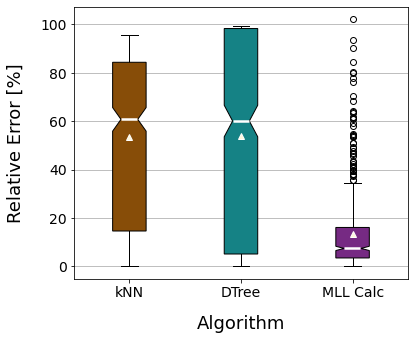
\includegraphics[width=\textwidth]{./chapters/exp1/sfcompo_boxplots_0null_pcterr_burn.png}
    \caption{Box plots of burnup percentage errors using zero-imputed null values.}
    \label{fig:burn0pct}
  \end{subfigure}
  \caption[Box plots of burnup regression of \acrshort{SFCOMPO} entries]
          {Box plots of burnup prediction errors and percentage errors for each 
           algorithm using two missing entry techniques: imputation with mean 
           values and with zero.}
  \label{fig:sfcoburn}
\end{figure}

\todo[inline]{BL: PHWR will build up Pu much more quickly so failure to detect
PHWR will cause problems.} The large ranges seen for the mean-imputed nulls
test set in Figure \ref{fig:burnimppct} are because of large overpredictions of
low burnups ($< 10\:GWd/MTU$), since a small number in the denominator will
yield a high percentage error. A large subset of the low burnup cases are
\gls{PHWR}s.  Their burnups are also unlikely to be predicted well because of
the inability of \gls{PHWR} reactors to be represented accurately with this
methodology.  Removing the \gls{PHWR} reactors from the results removes all
outliers with percentage errors larger than 1750\%. That is still a very high
relative error, but there are other low burnup cases in the database.  Removing
\gls{PHWR}s does not significantly alter the zero-imputed nulls results in
Figure \ref{fig:burn0pct}.

The range of percentage errors for the zero-imputed nulls test set in Figure
\ref{fig:burn0pct} tells a different story. There is only one case (an
\gls{MLL} outlier) that is above 100\% error.  While the absolute errors for
the scikit-learn algorithms in Figure \ref{fig:burn0} span a larger range than
their counterparts in Figure \ref{fig:burnimp}, their relative errors remain
within $0-100\%$. The only case that predicts the burnup well is the \gls{MLL}
method with the zero-imputed missing values treatment of the \gls{SFCOMPO} test
set, but about 8\% of the test cases are outliers.  If the best-case median
error of $1.7\:GWd/MTU$ in Table \ref{tbl:sfcoburn} were to also correspond to
a lower relative error, then that would be an acceptable result.  However,
while the \gls{MLL} calculations have a percentage error below 20\% at the 75\%
quartile, the non-outlier data reaches almost 40\% and the 8\% of the data
reaches 100\%.

\begin{figure}[!htb]
  \centering
  \begin{subfigure}[b]{\textwidth}
    \centering
    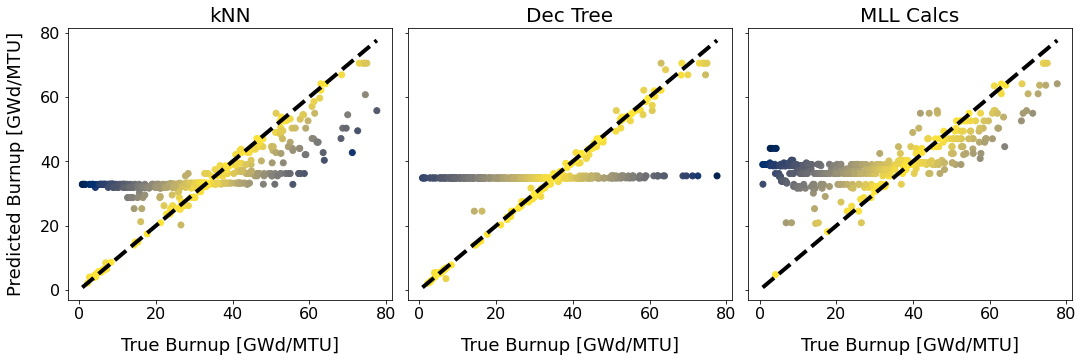
\includegraphics[width=\textwidth]{./chapters/exp1/sfcompo_truey_vs_predy_impnull__burn.png}
    \caption{True versus predicted burnup using mean-imputed null values.}
    \label{fig:yvy_burnimp}
  \end{subfigure}
  \vskip\baselineskip
  \begin{subfigure}[b]{\textwidth}
    \centering
    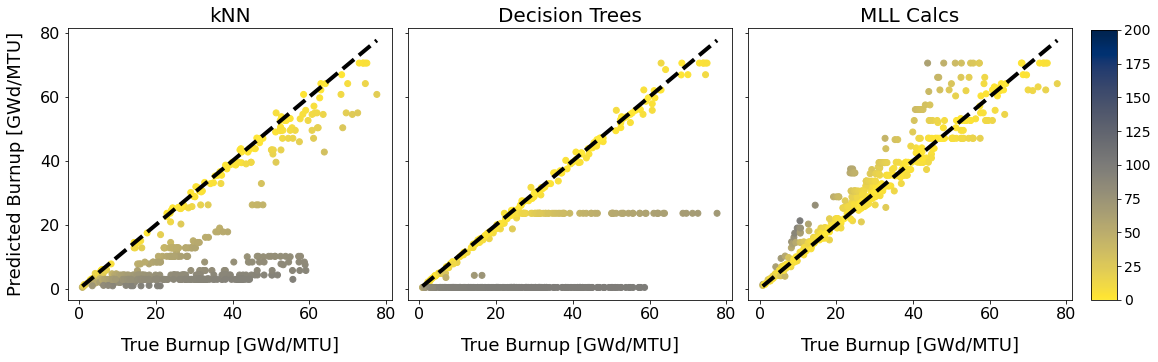
\includegraphics[width=\textwidth]{./chapters/exp1/sfcompo_truey_vs_predy_0null__burn.png}
    \caption{True versus predicted burnup using zero-imputed null values.}
    \label{fig:yvy_burn0}
  \end{subfigure}
  \caption[True versus predicted burnup of \acrshort{SFCOMPO} test cases]
          {True versus predicted burnup for each algorithm using two missing 
           entry techniques for \acrshort{SFCOMPO}: imputation with mean 
           values and with zero.}
  \label{fig:yvy_sfcoburn}
\end{figure}

To better understand the high errors in Figure \ref{fig:sfcoburn} and
especially the relative error outliers, Figure \ref{fig:yvy_sfcoburn} presents
the plots of the true burnup versus the predicted burnup for each test sample
in \gls{SFCOMPO} for each algorithm and both imputation techniques.  The
colorbar is the percentage error and was chosen with the range up to 200\%.
This is in order to show the difference between the large errors below the
diagonal line generally having a maximum error of 100\%, whereas the
mispredicted low-burnup cases have errors exceeding 200\%.  First, Figure
\ref{fig:yvy_burnimp} shows that all of the large errors are centered around a
certain predicted burnup range, $30-40\:GWd/MTU$. This is happening because
mean imputation technique is being applied to a data set where the measurements
likely only exist for a small range of burnup values, and each test sample is
likely to have many missing values.  The very large relative errors from Figure
\ref{fig:burnimppct} ($200\%-5000\%$) are clustered in the same place for all
three algorithms.  For Figure \ref{fig:yvy_burn0}, the large-error predictions
are shown clustered towards the bottom. This makes sense for the scikit-learn
algorithms since the zero measurements are easily interpreted as low burnup. Of
course, this is not the case for the \gls{MLL} calculations since the zero
values are filtered. 

Overall, the absolute errors in Table \ref{tbl:sfcoburn} tell a much more
encouraging story than the box plots in Figure \ref{fig:sfcoburn}, so
investigating beyond the mean and median absolute errors was necessary to show
the real picture of this unique testing scenario. The additional details
provided by directly plotting the true versus predicted burnup in Figure
\ref{fig:yvy_sfcoburn} is crucial in understanding how the null-value handling
methods impacted the results.

\noindent \textbf{\gls{U235} Enrichment}

For both reactor type classification and burnup regression, the zero-imputed
nulls test set predicted by \gls{MLL} calculations far outperform all other
algorithm/test set scenarios. However, the enrichment regression results break
this trend.  Table \ref{tbl:sfcoenri} shows that decision trees outperform the
other methods, and furthermore, there isn't a large difference in performance
between the two test sets, especially seeing that the median absolute error is
the same for both test sets.  The other two algorithms follow their previous
behavior: moving from mean-imputed nulls to zero-imputed nulls,
\textit{k}-nearest neighbors has worse performance and \gls{MLL} calculations
has better performance.

\begin{table}[!htb]
  \centering
  \begin{tabular}{@{}m{1.5in}llllll@{}}
    \toprule
                     & \multicolumn{3}{m{2in}}{Mean Errors [$\%\:{}^{235}\text{U}$]} 
                     & \multicolumn{3}{l}{Median Errors [$\%\:{}^{235}\text{U}$]} 
                     \\ \toprule
    Null Handling    & kNN  & DTree & MLL  & kNN   & DTree & MLL    \\ \midrule
    Mean Imputation  & 0.72 & 0.31  & 1.25 & 0.50  & 0.22  & 1.13   \\
    Zero Imputation  & 1.67 & 0.36  & 0.49 & 2.02  & 0.22  & 0.35   \\ \bottomrule
  \end{tabular}
  \caption[Performance of enrichment regression of \acrshort{SFCOMPO} entries]
          {Mean and median errors for enrichment prediction of the \gls{SFCOMPO} 
           test cases.}
  \label{tbl:sfcoenri}
\end{table}

The mean and median absolute errors are also visible with more statistical
information in the box plots in Figure \ref{fig:sfcoenri}. The outliers for
decision trees and \gls{MLL} calculations are 30 and 16 for the mean-imputed nulls
in Figure \ref{fig:enriimp}, respectively. So although decision trees provides
a typically low absolute error, the outliers reach nearly as far as the spread
of \textit{k}-nearest neighbors. The number of outliers for the zero-imputed nulls
results in Figure \ref{fig:enri0} are 45 and 16 for decision trees and
\gls{MLL} calculations, respectively.  The spread of the outliers for these
algorithms is similar to the previous figure, but \textit{k}-nearest neighbors
has a larger spread of absolute error.

\begin{figure}[!htb]
  \centering
  \begin{subfigure}[b]{0.49\textwidth}
    \centering
    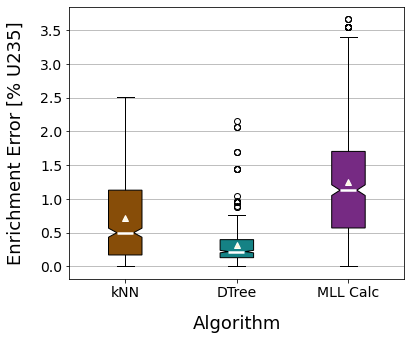
\includegraphics[width=\textwidth]{./chapters/exp1/sfcompo_boxplots_impnull_enri.png}
    \caption{Box plots of enrichment errors using mean-imputed null values.}
    \label{fig:enriimp}
  \end{subfigure}
  \hfill
  \begin{subfigure}[b]{0.49\textwidth}
    \centering
    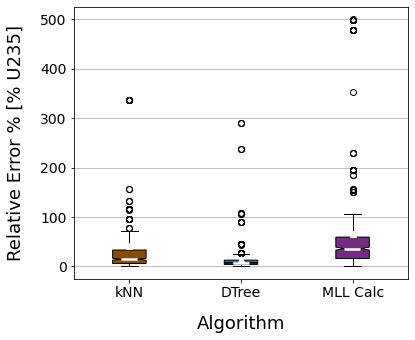
\includegraphics[width=\textwidth]{./chapters/exp1/sfcompo_boxplots_impnull_pcterr_enri.png}
    \caption{Box plots of enrichment percentage errors using mean-imputed null values.}
    \label{fig:enriimppct}
  \end{subfigure}
  \vskip\baselineskip
  \begin{subfigure}[b]{0.49\textwidth}
    \centering
    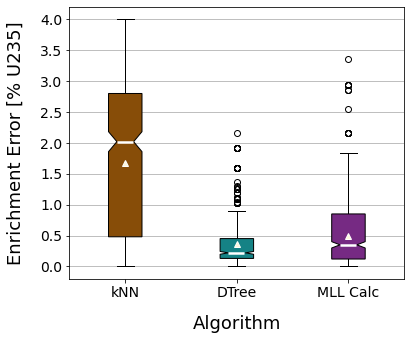
\includegraphics[width=\textwidth]{./chapters/exp1/sfcompo_boxplots_0null_enri.png}
    \caption{Box plots of enrichment errors using zero-imputed null values.}
    \label{fig:enri0}
  \end{subfigure}
  \hfill
  \begin{subfigure}[b]{0.49\textwidth}
    \centering
    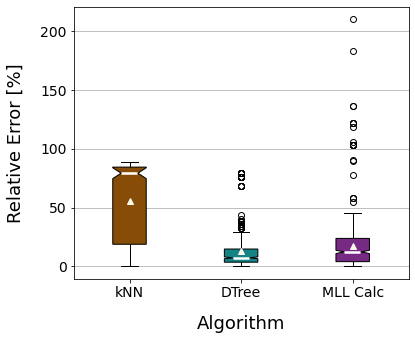
\includegraphics[width=\textwidth]{./chapters/exp1/sfcompo_boxplots_0null_pcterr_enri.png}
    \caption{Box plots of enrichment percentage errors using zero-imputed null values.}
    \label{fig:enri0pct}
  \end{subfigure}
  \caption[Box plots of enrichment regression of \acrshort{SFCOMPO} entries]
          {Box plots of enrichment prediction errors and percentage errors for 
           each algorithm using two missing entry techniques: imputation with 
           mean values and with zero.}
  \label{fig:sfcoenri}
\end{figure}

Again, a look at the relative errors gives a different sense of these results.
Figures \ref{fig:enriimppct} and \ref{fig:enri0pct} present the percent error
statistics for the mean-imputed nulls and zero-imputed nulls test sets,
respectively.  In Figure \ref{fig:enriimppct} there are 57, 39, and 49 outliers
for the \textit{k}-nearest neighbors, decision trees, and \gls{MLL}
calculations, respectively.  In Figure \ref{fig:enri0pct} there are 44 and 23
outliers for the decision trees and \gls{MLL} calculations, respectively.

As with the burnup regression, the high percentage errors are caused by a large
overprediction of enrichments that are of low value. All of the \gls{PHWR}s fit
into this category, and removing them from the results removes the outliers
with the highest errors from the mean-imputed nulls results in Figure
\ref{fig:enriimppct}, leaving a maximum of 250\% enrichment error. This is
still a high maximum error because there are other low enrichments not
belonging to the \gls{PHWR} class that remain overpredicted.  As with the
burnup, removing \gls{PHWR}s does not significantly alter the zero-imputed
nulls results in Figure \ref{fig:enri0pct}.

Unlike the case with burnup, the decision trees algorithm gives a better
performance that is null handling-independent than the other algorithm/test set
scenarios. Although there was a slightly worse mean absolute error for the
zero-imputed nulls test set (the median absolute error was the same), the
relative error remains below 100\% for all outliers, as seen in Figure
\ref{fig:enri0pct}.  This makes the decision trees algorithm with the
zero-imputed nulls test set the best performing case for enrichment regression.
It is an unexpected result to have either one of the scikit algorithms
outperform \gls{MLL} calculations for the zero-imputed nulls test set, since
they tended to have lower errors using the mean-imputed nulls test set. But
decision trees are capable of ignoring certain features if they do not lower
the node impurity (recall Equations \ref{eq:gini} and \ref{eq:mse}), so it is
not an unexpected result without an explanation.

\begin{figure}[!htb]
  \centering
  \begin{subfigure}[b]{\textwidth}
    \centering
    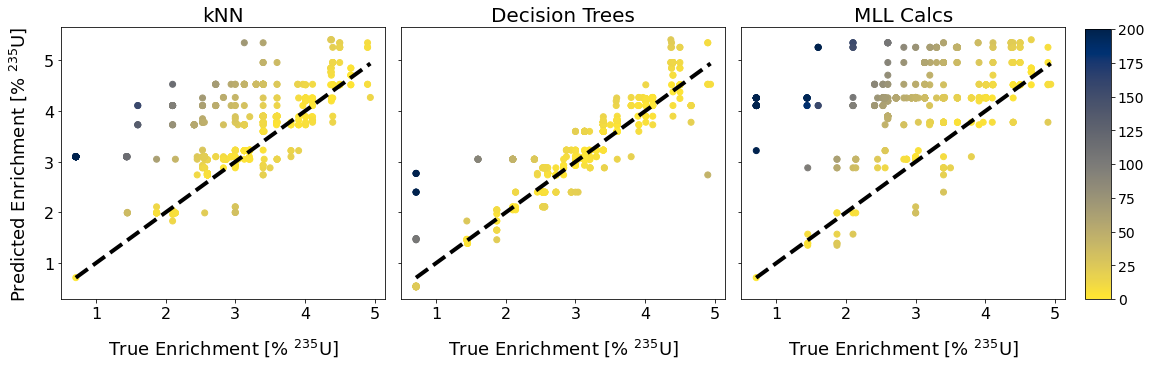
\includegraphics[width=\textwidth]{./chapters/exp1/sfcompo_truey_vs_predy_impnull__enri.png}
    \caption{True versus predicted enrichment using mean-imputed null values.}
    \label{fig:yvy_enriimp}
  \end{subfigure}
  \vskip\baselineskip
  \begin{subfigure}[b]{\textwidth}
    \centering
    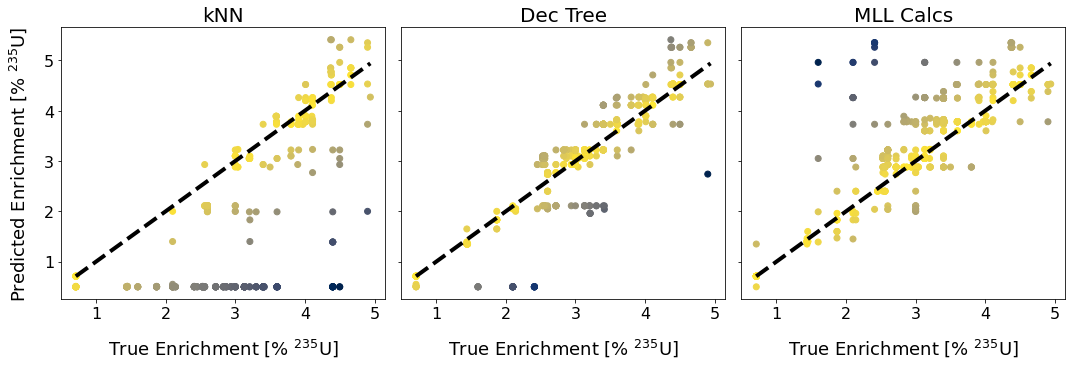
\includegraphics[width=\textwidth]{./chapters/exp1/sfcompo_truey_vs_predy_0null__enri.png}
    \caption{True versus predicted enrichment using zero-imputed null values.}
    \label{fig:yvy_enri0}
  \end{subfigure}
  \caption[True versus predicted enrichment of \acrshort{SFCOMPO} test cases]
          {True versus predicted enrichment for each algorithm using two missing
           entry techniques for \acrshort{SFCOMPO}: imputation with mean 
           values and with zero.}
  \label{fig:yvy_sfcoenri}
\end{figure}

To better understand the high errors in Figure \ref{fig:sfcoenri} and
especially the relative error outliers, Figure \ref{fig:yvy_sfcoenri} presents
the plots of the true \gls{U235} enrichment versus the predicted \gls{U235}
enrichment for each test sample in \gls{SFCOMPO} for each algorithm and both
imputation techniques.  The colorbar is the percentage error and was chosen
with the range up to 200\%.  This is in order to show the difference between
the large errors below the diagonal line generally having a maximum error of
100\%, whereas the errors above the diagonal line can exceed 200\%.  First,
Figure \ref{fig:yvy_enriimp} does not follow the same pattern as its burnup
counterpart (Figure \ref{fig:yvy_burnimp}) where the predictions are clustered
at a certain level due to the mean imputation.  There is still a general trend
of lower levels of enrichment being over-predicted, which are the large
relative error cases.  This is not happening because the missing values are not
strong enrichment indicators, because there is a clear effect when they are
imputed with zero, as shown in Figure \ref{fig:yvy_enri0}.  Here, the
large-error predictions are shown clustered towards the bottom for the
scikit-learn algorithms.  As with burnup (Figure \ref{fig:yvy_burn0}), this is
not the case for the \gls{MLL} calculations since the zero values are filtered. 

Overall, as with the case with burnup, the mean and median absolute errors in
Table \ref{tbl:sfcoenri} tell a much more encouraging story than the box plots
in Figure \ref{fig:sfcoenri}.  Looking at the spread of absolute errors and the
large relative errors gives the sense that the enrichment predictions are quite
poor as a whole. This does not mean it is hopeless; the decision tree approach
here warrants more investigation since the spread of errors in Figure
\ref{fig:enri0} is under $1.0\%\:{}^{235}\text{U}$. The additional details
provided by directly plotting the true versus predicted enrichment in Figure
\ref{fig:yvy_sfcoenri} is helpful in understanding how the null-value handling
methods impacted the results.

